% Sistema primado rotado un ángulo θ_0 (libro fig. 4.1)
\documentclass[border=4pt]{standalone}
\usepackage{tikz}
\usetikzlibrary{arrows.meta, calc}
\begin{document}
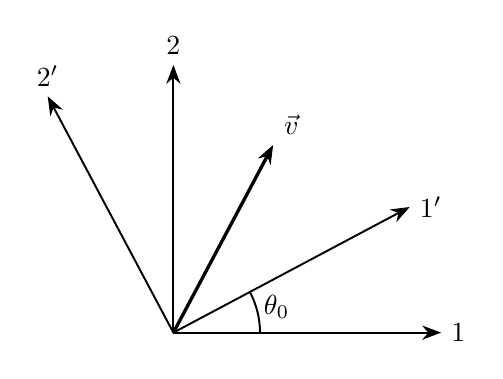
\begin{tikzpicture}[>={Stealth[length=2.4mm]}, line width=0.7pt]
  % sistema no primado
  \draw[->] (0,0)--(3.4,0) node[right]{$1$};
  \draw[->] (0,0)--(0,3.4) node[above]{$2$};
  % sistema primado (rotado θ_0)
  \draw[->] (0,0)--(28:3.4) node[right]{$1'$};
  \draw[->] (0,0)--(118:3.4) node[above]{$2'$};
  \draw (1.1,0) arc (0:28:1.1); \node at (14:1.35){$\theta_0$};
  % vector v (el mismo en ambos sistemas)
  \draw[->, line width=1.2pt] (0,0)--(62:2.7) node[above right]{$\vec v$};
\end{tikzpicture}
\end{document}
